\subsection*{Contexte}

On a vu que si \({(X_n)}_{n\in\bb N}\) était une suite
i.i.d.\ de variables aléatoires réelles intégrables,
alors
\begin{equation*}
    \frac{X_1 + \cdots + X_n}{n} \cvpsn \bb E[X_1]
\end{equation*}

\subsection*{Question}

Que dire de l'écart entre \(\frac{X_1 + \cdots + X_n}{n}\) et \(\bb E[X_1]\)?

\section{Convergence en loi}

\subsection*{Notation}

Dans cette section, \(C_b^0(\bb R)\) l'ensemble
des fonctions \(h:\bb R\to\bb R\) continues bornées
munies de la norme
\begin{equation*}
    \nn{h}_{\infty} = \sup_{x\in\bb R} |h(x)|
\end{equation*}

\subsection{Définition et premiers exemples}

\begin{definition}
    Soit \({(X_n)}_{n\geq 1}\) une suite de variables aléatoires réelles
    et \(X\) une variable aléatoire réelle. On dit que \({(X_n)}_{n\geq 1}\)
    \defemph{converge en loi} vers \(X\) si pour tout \(h\in C_b^0(\bb R)\),
    on a
    \begin{equation*}
        \bb E[h(X_n)] \cvn \bb E[h(X)]
    \end{equation*}
    On note alors
    \begin{equation*}
        X_n \cvlawn X
    \end{equation*}
    ou bien
    \begin{equation*}
        X_n \cvdn X
    \end{equation*}
\end{definition}

\begin{remark}\,
    \begin{enumerate}
        \item On peut étendre cette définition à des vecteurs aléatoires
        en prenant des fonctions \(h:\bb R^d\to\bb R\) continues bornées.

        \item Cette notion de convergence ne fait intervenir que la loi
        des variables aléatoires considérées. Dans la limite, on peut donc
        remplacer \(X\) par n'importe quelle variable aléatoire \(Y\) de
        même loi.\\
        Si \(\mu\) désigne la loi de \(X\), on notera alors
        \begin{equation*}
            X_n \cvlawn \mu
        \end{equation*}
    \end{enumerate}
\end{remark}

\begin{example}
    Soit \({(X_n)}_{n\geq 1}\) une suite de variables aléatoires
    telles que pour tout \(n\geq 1\), \(X_n\) suit une loi uniforme
    sur \(\left\{0,\frac1n,\frac2n,\ldots,\frac{n-1}{n},1\right\}\).
    % graph of X1,X2 and X3 as a line with points on every i/n:
    % X1: 0, 1
    % X2: 0, 1/2, 1
    % X3: 0, 1/3, 2/3, 1
    \begin{center}
        \begin{tikzpicture}
            % lines
            \draw (-2.5,2) -- (2.5,2);
            \draw (-2.5,1) -- (2.5,1);
            \draw (-2.5,0) -- (2.5,0);

            % 0s
            \node[below] at (-2.25,2) {\(0\)};
            \node[below] at (-2.25,1) {\(0\)};
            \node[below] at (-2.25,0) {\(0\)};

            % 1s
            \node[below] at (2.25,2) {\(1\)};
            \node[below] at (2.25,1) {\(1\)};
            \node[below] at (2.25,0) {\(1\)};

            % bonus points for X1
            %%

            % points for X2
            \node[below] at (0,1) {\(\frac12\)};

            % points for X3 %-2.5+1.6666666666666667 = -0.8333333333333333
            \node[below] at (-0.8333,0) {\(\frac13\)};
            \node[below] at (0.8333,0) {\(\frac23\)};

            % probabilities for all points above
            \node[above] at (-2.25,2) {\(\frac12\)};
            \node[above] at (-0.8333,0) {\(\frac14\)};
            \node[above] at (0.8333,0) {\(\frac14\)};
            \node[above] at (2.25,2) {\(\frac12\)};




        \end{tikzpicture}
    \end{center}

    La loi de \(X_n\) est donnée par
    \begin{equation*}
        \bb P(X_n = k) = \frac1{n+1} \quad \text{pour } k=0,1,\ldots,n
    \end{equation*}
    Soit \(h\in C_b^0(\bb R)\). On a
    \begin{equation*}
        \begin{aligned}
            \bb E[h(X_n)] 
            &= \sum_{k=0}^n h\left(\frac kn\right) \frac1{n+1}\\
            &= \frac1{n+1} \sum_{k=0}^n h\left(\frac kn\right)\\
            &\cvn \int_0^1 h(x) \der x
        \end{aligned}
    \end{equation*}
    par convergence des sommes de Riemann. On considère une variable aléatoire
    \(X\) suivant une loi uniforme sur \([0,1]\). On a alors
    \begin{equation*}
        \bb E[h(X)] = \int_0^1 h(x) \der x
    \end{equation*}
    Donc pour tout \(h\in C_b^0(\bb R)\), on a
    \begin{equation*}
        \bb E[h(X_n)] \cvn \bb E[h(X)]
    \end{equation*}
    et donc
    \begin{equation*}
        X_n \cvlawn X
    \end{equation*}
    Pkus simplement, on écrit
    \begin{equation*}
        X_n \cvlawn \mathcal U([0,1])
    \end{equation*}
\end{example}

\begin{example}
    Soit \({(X_n)}_{n\geq 1}\) une suite de variables aléatoires
    telle que \(X_n\sim\mathcal N(0,\sigma_n^2)\) avec \(\sigma_n> 0\)
    et \(\sigma_n\cvn 0\). On a alors
    \begin{equation*}
        \begin{aligned}
            \bb E[h(X_n)]
            &= \int_{\bb R} h(x) \frac{e^{-\frac{x^2}{2\sigma_n^2}}}{\sqrt{2\pi}\sigma_n}  \der x\\
            \smol{\(y=\frac{x}{\sigma_n}\)}&= \int_{\bb R} \underbrace{h(\sigma_n y) \frac{e^{-\frac{y^2}{2}}}{\sqrt{2\pi}}}_{g_n(y)\cvn h(0) \frac{e^{-\frac{y^2}{2}}}{\sqrt{2\pi}}} \der y\\
        \end{aligned}
    \end{equation*}
    Comme \(|g_n(y)|\leq \nn{h}_{\infty} \frac{e^{-\frac{y^2}{2}}}{\sqrt{2\pi}}\), on
    applique le théorème de convergence dominée pour obtenir
    \begin{equation*}
        \bb E[h(X_n)] \cvn \int_{\bb R} h(0) \frac{e^{-\frac{y^2}{2}}}{\sqrt{2\pi}} \der y= h(0)
    \end{equation*}
    Soit \(X\) de loi \(\delta_n\). On a montré que pour tout \(h\in C_b^0(\bb R)\),
    \begin{equation*}
        \bb E[h(X_n)] \cvn \bb E[h(X)]=h(0)
    \end{equation*}
    donc
    \begin{equation*}
        X_n \cvlawn X
    \end{equation*}
    ce qu'on réécrit
    \begin{equation*}
        X_n \cvlawn \delta_0
    \end{equation*}
\end{example}

\subsection{Deux cas particuliers}

\subsubsection{Loi sur \(\bb N\)}

\begin{proposition}
    Une suite de variables aléatoires \({(X_n)}_{n\geq 1}\) converge 
    vers une variable aléatoire \(X\) à valeurs dans \(\bb N\) si et seulement
    si pour tout \(k\in\bb N\), on a
    \begin{equation*}
        \bb P(X_n = k) \cvn \bb P(X = k)
    \end{equation*}
\end{proposition}

\begin{proof}\,
    \begin{itemize}[\ptr{}]
        \item Sens direct:\\
        Supposons que \(X_n \cvlawn X\). Soit \(k\in\bb N\). On sait que
        pour tout \(h\in C_b^0(\bb R)\), on a
        \begin{equation*}
            \begin{aligned}
                \bb E[h(X_n)]
                &= \sum_{j=0}^{+\infty} h(j) \bb P(X_n = j)\\
                &\cvn \bb E[h(X)]\\
                &= \sum_{j=0}^{+\infty} h(j) \bb P(X = j)
            \end{aligned}
        \end{equation*}
        On prend alors \(h\) telle que \(h(k) = 1\) et \(h(j) = 0\) pour
        \(j\neq k\).
        % graph of h 0 everywhere except at k where it is 1, forms a 
        % triangle with base 2 centered at k, height 1
        %\begin{center}
        %    \begin{tikzpicture}
        %        % axes
        %        \draw[->] (-2,0) -- (2,0);
        %        \draw[->] (0,-0.5) -- (0,1.5);
%
        %        % h
        %        \draw (-1,0) -- (1,1) -- (1,0);
%
        %        % labels
        %        \node[below] at (1,0) {\(k\)};
        %        \node[left] at (0,1) {\(1\)};
        %    \end{tikzpicture}
        %\end{center}
        Ainsi,
        \begin{equation*}
            \bb E[h(X_n)] = \sum_{j=0}^{+\infty} h(j) \bb P(X_n = j) = \bb P(X_n = k) 
        \end{equation*}
        et de même pour \(X\), donc
        \begin{equation*}
            \bb P(X_n = k) \cvn \bb P(X = k)
        \end{equation*}

        \item Réciproque vue plus tard.
    \end{itemize}
\end{proof}

\begin{example}
    Approximation binomiale de la loi de Poisson. Soit \({(X_n)}_{n\geq 1}\)
    une suite de variables aléatoires de loi \(X_n\sim\mathcal B(n,p_n)\) avec
    \(n p_n\cvn \theta>0\). Montrons que \(X_n \cvlawn X\) où \(X\sim\mathcal P(\theta)\).

    Soit \(k\in\bb N\). On a
    \begin{equation*}
        \begin{aligned}
            \bb P(X_n = k)
            &= \binom{n}{k} p_n^k {(1-p_n)}^{n-k}\\
            &= \frac{n!}{k!(n-k)!} p_n^k {(1-p_n)}^{n-k}\\
            &= \frac{n(n-1)\cdots(n-k+1)}{k!} {\left(\frac{p_n}{1-p_n}\right)}^k {(1-p_n)}^n\\
            &\cvn \frac{\theta^k}{k!} e^{-\theta}
        \end{aligned}
    \end{equation*}
    Bref, on obtient
    \begin{equation*}
        \bb P(X_n = k) \cvn \frac{\theta^k}{k!} e^{-\theta}= \bb P(X = k)
    \end{equation*}
    donc
    \begin{equation*}
        X_n \cvlawn X
    \end{equation*}
    ou encore
    \begin{equation*}
        X_n \cvlawn \mathcal P(\theta)
    \end{equation*}
\end{example}

\subsubsection{Loi à densité sur \(\bb R\)}

\begin{proposition}
    Soit \({(X_n)}_{n\geq 1}\) une suite de variables aléatoires
    telles que \(X_n\) a pour densité \(f_n\) et \(X\) 
    une variable aléatoire de densité \(f\). Si
    \begin{equation*}
        \quad f_n \cvn f,\quad \lambda\text{-p.p.}
    \end{equation*}
    alors
    \begin{equation*}
        X_n \cvlawn X
    \end{equation*}
\end{proposition}

\begin{proof}
    On veut montrer que pour tout \(h\in C_b^0(\bb R)\), on a
    \begin{equation*}
        \begin{aligned}
            \bb E[h(X_n)]
            &= \int_{\bb R} h(x) f_n(x) \der \lambda_1(x)\\
            &\cvn \bb E[h(X)]\\
            &= \int_{\bb R} h(x) f(x) \der \lambda_1(x)
        \end{aligned}
    \end{equation*}
    le théorème de convergence dominée ne s'applique pas.

    On applique le lemme de Fatou à la suite de fonctions
    positives mesurables
    \begin{equation*}
        g_n(x) = \min(f_n(x),f(x)) = \frac{f_n(x)+f(x)-|f_n(x)-f(x)|}{2}
    \end{equation*}
    On a
    \begin{equation*}
        \int_{\bb R} \liminf_{n\to+\infty} g_n(x) \der \lambda_1(x) \leq \liminf_{n\to+\infty} \int_{\bb R} g_n(x) \der \lambda_1(x)
    \end{equation*}
    Par ailleurs, on a
    \begin{equation*}
        \begin{aligned}
            \int_{\bb R} g_n(x) \der \lambda_1(x)
            &= \frac12 \int_{\bb R} f_n(x) \der \lambda_1(x) + \frac12 \int_{\bb R} f(x) \der \lambda_1(x) - \frac12 \int_{\bb R} |f_n(x)-f(x)| \der \lambda_1(x)\\
            &= 1 - \frac12 \int_{\bb R} |f_n(x)-f(x)| \der \lambda_1(x)
        \end{aligned}
    \end{equation*}
    Bref, on a
    \begin{equation*}
        0\leq \liminf_{n\to+\infty} \int_{\bb R} |f_n(x)-f(x)| \der \lambda_1(x)
    \end{equation*}
    Ainsi, on a
    \begin{equation*}
        \limsup_{n\to+\infty} \int_{\bb R} |f_n(x)-f(x)| \der \lambda_1(x) \leq 0
    \end{equation*}
    et donc
    \begin{equation*}
        \lim_{n\to+\infty} \int_{\bb R} |f_n(x)-f(x)| \der \lambda_1(x) = 0
    \end{equation*}
    Par suite, on en déduit que
    \begin{equation*}
        \n{\bb E[h(X_n)] - \bb E[h(X)]} \leq \nn{h}_{\infty} \int_{\bb R} |f_n(x)-f(x)| \der \lambda_1(x) \cvn 0
    \end{equation*}
\end{proof}

\begin{example}
    Si \(X\sim E(\theta_n)\) avec \(\theta_n\cvn \theta\), alors 
    les densités de \(X_n\) vérifient
    \begin{equation*}
        f_n(x) = \theta_n e^{-\theta_n x} \cvn \theta e^{-\theta x} = f(x)
    \end{equation*}
    où \(f\) est la densité d'une loi exponentielle de paramètre \(\theta\).
    Donc
    \begin{equation*}
        X_n \cvlawn \mathcal E(\theta)
    \end{equation*}
\end{example}

\subsection{Lien avec les autres modes de convergence}

\begin{proposition}\,
    Soit \({(X_n)}_{n\geq 1}\) une suite de variables aléatoires
    et \(X\) une variable aléatoire. Alors
    \begin{equation*}
        X_n\cvpn X \implies X_n\cvlawn X
    \end{equation*}
\end{proposition}

\begin{proof}
    Soit \(h\in C_b^0(\bb R)\) et \(\varepsilon>0\). On a
    \begin{equation*}
        \underbrace{\n{\bb E[h(X_n)] - \bb E[h(X)]}}_{=\alpha} \leq \bb E[\n{h(X_n)-h(X)}]
    \end{equation*}
    où
    \begin{equation*}
        \begin{aligned}
            \alpha 
            &= \bb E[\n{h(X_n)-h(X)}\one_{\n{h(X_n)-h(X)}\geq \varepsilon}]\quad \color{red}(1)\\
            \color{black}&+ \bb E[\n{h(X_n)-h(X)}\one_{\n{h(X_n)-h(X)}< \varepsilon}]\quad \color{blue}(2)
        \end{aligned}
    \end{equation*}
    On a alors
    \begin{equation*}
        \begin{aligned}
            \color{red}(1) \color{black}
            &\leq \bb E[\left(\n{h(X_n)}+\n{h(X)}\right)\one_{\n{h(X_n)-h(X)}\geq \varepsilon}]\\
            &\leq 2 \nn{h}_{\infty} \underbrace{\bb P(\n{h(X_n)-h(X)}\geq \varepsilon)}_{\leq\varepsilon}\\
        \end{aligned}
    \end{equation*}
    car \(h(X_n)\cvpn h(X)\).
    De même,
    \begin{equation*}
        \color{blue}(2) \color{black}
        \leq \bb E[\varepsilon \one_{\n{h(X_n)-h(X)}< \varepsilon}]\leq \varepsilon
    \end{equation*}
    Bref, on a
    \begin{equation*}
        \n{\bb E[h(X_n)] - \bb E[h(X)]} \leq \varepsilon(1 + 2\nn{h}_{\infty})
    \end{equation*}
    donc \(\bb E[h(X_n)] \cvn \bb E[h(X)]\), donc \(X_n\cvlawn X\).
\end{proof}

\begin{example}[Réciproque fausse]
    On prend
    \begin{equation*}
        X\sim \mathcal B\left(\frac12\right),\quad X_n = X \quad\text{pour tout } n\geq 1
    \end{equation*}
    Alors, on a bien \(X_n\cvlawn X\).\\
    Remarquons que \(Y = 1-X\sim \mathcal B\left(\frac12\right)\) donc on a ausse
    \(X_n\cvlawn Y\) (ce qu'on écrit \(X_n\cvlawn \mathcal B\left(\frac12\right)\)).\\
    Or, on a
    \begin{equation*}
        \n{X_n - Y} = \n{X-(1-X)} = \n{2X-1} = 1
    \end{equation*}
    et donc \({(X_n)}_{n\geq 1}\) ne converge pas en probabilité vers \(Y\).
\end{example}

\begin{proposition}
    Si \(X_n\cvlawn c\) où \(c\) est une constante, alors \(X_n\cvpn c\).
\end{proposition}

\begin{proof}
    Soit \(\varepsilon>0\). On a
    \begin{equation*}
        \begin{aligned}
            \bb P(\n{X_n-c}\geq \varepsilon)
            &= \bb E[\one_{\n{X_n-c}\geq \varepsilon}]\\
            &\leq \bb E[h(X_n)]\cvn \bb E[h(c)] = 0
        \end{aligned}
    \end{equation*}
    pour un \(h\) judicieusement choisi.\\
    On choisit alors \(h(x) = \min(1,\frac{\n{x-c}}{\varepsilon})\). On a
    % insert tikz graph here as follows:
    % 1 between -1 and 1, down to 0 at 2, up to 1 at 3 stays at 1 until 5
    % "c" at 2, "c+\varepsilon" at 3, "c-\varepsilon" at 1, 
    % function above in blue, following function shifted by 0.05 in height in orange
    % same as above but 1 at [...,-1], 0 from ]-1,1[, 1 at [1,...]
    % h in blue, \one_{\n{X_n-c}\geq \varepsilon} in orange
    \begin{center}
        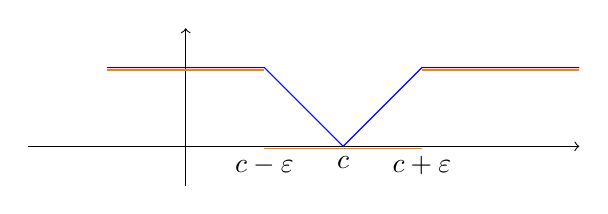
\begin{tikzpicture}
            % axes
            \draw[->] (-2,0) -- (5,0);
            \draw[->] (0,-0.5) -- (0,1.5);
%
            % h
            \draw[blue] (-1,1) -- (1,1) -- (2,0) -- (3,1) -- (5,1);
            \draw[orange] (-1,0.97) -- (1,0.97);
            \draw[orange] (3,0.97) -- (5,0.97);
            \draw[orange] (1,-0.03) -- (3,-0.03);
%
            % labels
            \node[below] at (1,0) {\(c-\varepsilon\)};
            \node[below] at (3,0) {\(c+\varepsilon\)};
            \node[below] at (2,0) {\(c\)};
        \end{tikzpicture}
    \end{center}
\end{proof}

\section{Caractérisation de la convergence en loi}

\subsection{Restriction des fonctions tests}

\subsubsection*{Notation}

On note \(\mathcal C_C^0(\bb R)\) l'ensemble des fonctions continues à support 
compact. Cet ensemble est dense pour la norme \(\nn{\cdot}_{\infty}\) dans \(C_b^0(\bb R)\).

\begin{proposition}
    Soit \({(X_n)}_{n\geq 1}\) une suite de variables aléatoires réelles
    et \(X\) une variable aléatoire réelle. Alors, 
    \begin{equation*}
        X_n\cvlawn X \iff \forall h\in \mathcal C_C^0(\bb R),\quad \bb E[h(X_n)] \cvn \bb E[h(X)]
    \end{equation*}

    De plus, si \(H\) est un ensemble de fonctions mesurables bornées tel que
    \(\mathcal C_C^0(\bb R)\subset \ol H\) (adhérence de \(H\) pour la norme
    \(\nn{\cdot}_{\infty}\)), et si \(\forall h\in H\), \(\bb E[h(X_n)] \cvn \bb E[h(X)]\),
    alors \(X_n\cvlawn X\).
\end{proposition}

\begin{proof}
    On montre l'équivalence.\\
    \begin{itemize}[\ptr{}]
        \item Sens direct: evident.

        \item Sens indirect:\\
        Soit \(h\in C_b^0(\bb R)\). Soit \(g_k\) la fonction dans \(\mathcal C_C^0(\bb R)\)
        définie par 
        % tikz graph -5,-4 =0, up to 1 at -3, stays 1 until 3, down to 0 at 4, 0 to 5
        % -(k+1) at -4, (k+1) at 4, -k at -3, k at 3
        % g_k in blue
        %\begin{center}
        %    \begin{tikzpicture}
        %        % axes
        %        \draw[->] (-5,0) -- (5,0);
        %        \draw[->] (0,-0.5) -- (0,1.5);
%
        %        % g_k
        %        \draw[blue] (-5,0) -- (-4,0) -- (-3,1) -- (3,1) -- (4,0) -- (5,0);
%
        %        % labels
        %        \node[below] at (-4,0) {\(-(k+1)\)};
        %        \node[below] at (-3,0) {\(-k\)};
        %        \node[below] at (3,0) {\(k\)};
        %        \node[below] at (4,0) {\(k+1\)};
        %    \end{tikzpicture}
        %\end{center}
        On obtient que \(g_k\cv 1\) et donc \(h_{g_k}\in \mathcal C_C^0(\bb R)\)
        vérifie \(h_{g_k}\cv h\). En particulier, pour tout \(k\geq 1\),
        \begin{equation*}
            \bb E[h_{g_k}(X_n)] \cvn \bb E[h_{g_k}(X)]
        \end{equation*}
        On écrit
        \begin{equation*}
            \n{\bb E[h(X_n) -h(X)]} 
            \leq \color{orange}\underbrace{\color{black}\n{\bb E[h(X_n) - h_{g_k}(X_n)]}}_{(1)} \color{black}
            + \color{verdant}\underbrace{\color{black}\n{\bb E[h_{g_k}(X_n) - h_{g_k}(X)]}}_{(2)} \color{black}
            + \color{blue}\underbrace{\color{black}\n{\bb E[h_{g_k}(X) - h(X)]}}_{(3)}
        \end{equation*}
        On a alors
        \begin{itemize}
            \item[\(\color{verdant}(2)\)] \(\leq\varepsilon\) pour \(n\) assez grand
            car \(h_{g_k}\in \mathcal C_C^0(\bb R)\),

            \item[\(\color{orange}(1)\)] \(\leq \bb E[\n{h-h_{g_k}}(X_n)]\leq \bb E[\nn{h-h_{g_k}}_{\infty}]=\nn{h-h_{g_k}}_{\infty}\cv 0\),

            \item[\(\color{blue}(3)\)] \(\leq \bb E[\n{h-h_{g_k}}(X)]\leq \nn{h-h_{g_k}}_{\infty}\cv 0\).
        \end{itemize}
        Pour le deuxième, on utilise la même technique en prenant \(h\in \mathcal C_C^0(\bb R)\)
        et \(g_k\in H\) telle que \(g_k\cv h\) pour \(\nn{\cdot}_\infty\)
    \end{itemize}
\end{proof}

\subsubsection*{Application} Preuve de
\begin{equation*}
    \bb P(X_n=k)\cvn \bb P(X=k) \implies X_n\cvlawn X
\end{equation*}
pour \(X_n\) et \(X\) des variables aléatoires à valeurs dans \(\bb N\).\\
(cf.\ proposition de la section 1.2.1)\\
Soit \(h\in \mathcal C_C^0(\bb R)\); \(h\) est nulle en dehors de \(\ff{-K,K}\). Alors
\begin{equation*}
    \begin{aligned}
        \bb E[h(X_n)]
        &= \sum_{k=0}^{+\infty} h(k) \bb P(X_n=k)\\
        &= \sum_{k=0}^{\lfloor K\rfloor} h(k) \bb P(X_n=k)\\
        &\cvn \sum_{k=0}^{\lfloor K\rfloor} h(k) \bb P(X=k)\\
        &= \bb E[h(X)]
    \end{aligned}
\end{equation*}
et donc \(X_n\cvlawn X\).

\subsection{Caractérisation via la fonction de répartition et la fonction caractéristique}

\subsubsection*{Rappel}
Si \(X\) est une variable aléatoire réelle, sa fonction de répartition \(F_X\)
est définie par
\begin{equation*}
    F_X(t) = \bb P(X\leq t) = \bb E[\one_{\of{-\infty,t}}(X)]
\end{equation*}

On sait que \(F_X\) est continue à droite et que
\begin{equation*}
    \bb P(X=t) = F_X(t) - \lim\limits_{\substack{\varepsilon\to 0\\ \varepsilon>0}} F_X(t-\varepsilon)
\end{equation*}
donc \(F_X\) est continue en \(t\) si et seulement si \(\bb P(X=t) = 0\).

\begin{proposition}
    \({(X_n)}_{n\geq 1}\) converge en loi vers une variable aléatoire \(X\)
    si et seulement si pour tout point de continuité \(t\) de \(F_X\), on a
    \begin{equation*}
        F_{X_n}(t) \cvn F_X(t)
    \end{equation*}
\end{proposition}

\begin{proof}
    Dans les grandes lignes, on a
    \begin{itemize}[\ptr{}]
        \item Sens direct:\\
        Supposons 
        \begin{equation*}
            \bb E[h(X_n)] \cvn \bb E[h(X)]
        \end{equation*}
        Ob va approcher \(\one_{\of{-\infty,t}}\) par une fonction
        continue bornée \(h\):
        % 3 functions:
        % fct 1: 1 from 0 to 1, 0 from 1 to 3, noted \one_{\of{-\infty,t}, orange
        % fct 2: 1 from 0 to 2, 0 from 2 to 3, noted \one_{\of{-\infty,t+\varepsilon}, blue
        % fct 3: 1 from 0 to 1, downslope to 0 at 2, 0 from 2 to 3, noted h, verdant
        % all 3 functions shifted by 0.05 in height
        % points t and t+\varepsilon marked on the x-axis
        %\begin{center}
        %    \begin{tikzpicture}
        %        % axes
        %        \draw[->] (-1,0) -- (4,0);
        %        \draw[->] (0,-0.5) -- (0,1.5);
%
        %        % functions
        %        \draw[orange] (0,1) -- (1,1) -- (1,0) -- (3,0);
        %        \draw[blue] (0,1) -- (2,1) -- (2,0) -- (3,0);
        %        \draw[verdant] (0,1) -- (1,1) -- (2,0) -- (3,0);
%
        %        % labels
        %        \node[below] at (1,0) {\(t\)};
        %        \node[below] at (2,0) {\(t+\varepsilon\)};
        %    \end{tikzpicture}
        %\end{center}

        On sait qu'il y a convergence de \(\bb E[h(X_n)]\) vers \(\bb E[h(X)]\)
        donc par encadrement il y a convergence de \(\bb E[\one_{\of{-\infty,t}}(X_n)]\)
        vers \(\bb E[\one_{\of{-\infty,t}}(X)]\)

        \item Sens indirect:\\
        On note \(D\) l'ensemble des points de discontinuité de \(F_X\) et
        on définit
        \begin{equation*}
            H=\{\one_{\of{a,b}},a<b,a,b\in\bb R\setminus D\}
        \end{equation*}
        On montre que
        \begin{itemize}[]
            \item \(\forall h\in H,\bb E[h(X_n)] \cvn \bb E[h(X)]\),
            \item \(\mathcal C_C^0(\bb R)\subset \ol H\).
        \end{itemize}
        et on applique la proposition précédente.
    \end{itemize}
\end{proof}

\begin{theorem}[de Lévy]
    On a
    \begin{equation*}
        X_n\cvlawn X \iff \forall t\in\bb R,\quad \varphi_{X_n}(t) \cvn \varphi_X(t)
    \end{equation*}
\end{theorem}

\begin{proof}
    admise, elle s'appuie sur l'injectivité de la transformée de Fourier
    de mesures.
\end{proof}

\section{Théorème central limite}

\subsubsection*{Rappel}
Si \({(X_n)}_{n\geq 1}\) est une suite de variables aléatoires \iid{}
dans \(L^1(\Omega,\scr F,\bb P)\), alors la loi forte des grands nombres
assure que
\begin{equation*}
    \ol{X_n} = \frac{X_1+\cdots+X_n}{n} =\frac{S_n}{n} \cvpsn \bb E[X_1]
\end{equation*}
Que dire alors de l'écart entre \(S_n\) et \(n\bb E[X_1]\)?\\

\begin{theorem}[central limite]
    Soit \({(X_n)}_{n\geq 1}\) une suite de variables aléatoires
    réelles \iid{} dans \(L^2(\Omega,\scr F,\bb P)\). On suppose que
    \(\sigma^2=\var(X_1)>0\). Alors
    \begin{equation*}
        \frac{S_n-n\bb E[X_1]}{\sigma\sqrt{n}} \cvlawn \mathcal N(0,1)
    \end{equation*}
\end{theorem}

\begin{remark}\,
    \begin{enumerate}
        \item Pour se souvenir de la normalisation, il suffit de 
        penser à centrer et réduire \(S_n\) avec
        \begin{equation*}
            \begin{aligned}
                \bb E[S_n] &= n\bb E[X_1]\\
                \var(S_n) &= n\var(X_1) = n\sigma^2
            \end{aligned}
        \end{equation*}

        \item On peut réécrire la convergence de diverses façons:
        \begin{equation*}
            \begin{aligned}
                \frac{S_n-n\bb E[X_1]}{\sqrt{n}} &\cvlawn \mathcal N(0,\sigma^2)\\
                \frac{\ol{X_n}-\bb E[X_1]}{\frac{\sigma}{\sqrt{n}}} &\cvlawn \mathcal N(0,1)\\
            \end{aligned}
        \end{equation*}

        \item La caractérisation de la convergence en loi via les fonctions de répartition
        donne:
        \begin{equation*}
            \forall x\in\bb R,\quad \bb P\left(\frac{S_n-n\bb E[X_1]}{\sigma\sqrt{n}}\leq x\right) \cvn \bb P(N\leq x) = \int_{-\infty}^x \frac{e^{-\frac{t^2}{2}}}{\sqrt{2\pi}} \der t
        \end{equation*}
        avec \(N\sim\mathcal N(0,1)\).\\
        Plus généralement, si \(a<b\), alors
        \begin{equation*}
            \bb P\left(a\leq \frac{S_n-n\bb E[X_1]}{\sigma\sqrt{n}}\leq b\right) \cvn \int_a^b \frac{e^{-\frac{t^2}{2}}}{\sqrt{2\pi}} \der t
        \end{equation*}
        On notera parfois
        \begin{equation*}
            \Phi(x) = \int_{-\infty}^x \frac{e^{-\frac{t^2}{2}}}{\sqrt{2\pi}} \der t = \bb P(N\leq x)
        \end{equation*}
    \end{enumerate}
\end{remark}

\begin{proof}
    On montre la convergence en loi via les fonctions caractéristiques.\\
    On suppose, quitte à remplacer \(X_k\) par \(X_k-\bb E[X_1]\), que les \(X_k\)
    sont centrées.\\
    Montrons que
    \begin{equation*}
        \frac{S_n}{\sigma\sqrt{n}} \cvlawn \mathcal N(0,1)
    \end{equation*}
    Montrons que
    \begin{equation*}
        \varphi_{\frac{S_n}{\sigma\sqrt{n}}}(t) \cvn \varphi_N(t) = e^{-\frac{t^2}{2}}
    \end{equation*}
    pour tout \(t\in\bb R\). On a
    \begin{equation*}
        \begin{aligned}
            \varphi_{\frac{S_n}{\sigma\sqrt{n}}}(t)
            &= \bb E[e^{it\frac{S_n}{\sigma\sqrt{n}}}]\\
            &= \bb E[e^{it\frac{X_1+\cdots+X_n}{\sigma\sqrt{n}}}]\\
            &= \bb E[e^{it\frac{X_1}{\sigma\sqrt{n}}}\cdots e^{it\frac{X_n}{\sigma\sqrt{n}}}]\\
            &= \bb E[e^{it\frac{X_1}{\sigma\sqrt{n}}}]\cdots \bb E[e^{it\frac{X_n}{\sigma\sqrt{n}}}]\\
            &= \bb {E[e^{it\frac{X_1}{\sigma\sqrt{n}}}]}^n
            &= {\varphi_{X_1}\left(\frac{t}{\sigma\sqrt{n}}\right)}^n 
        \end{aligned}
    \end{equation*}
    Comme les \(X_k\) sont dans \(L^2(\Omega,\scr F,\bb P)\), \(\varphi_{X_1}\) est
    dans \(\mathscr C^2(\bb R, \bb C)\) avec
    \begin{equation*}
        \begin{aligned}
            & \varphi_{X_1}'(0)=i\bb E[X_1]=0,\\
            & \varphi_{X_1}''(0)=-\bb E[X_1^2]=-\sigma^2
        \end{aligned}
    \end{equation*}
    Un développement limité en 0 de \(\varphi_{X_1}\) donne
    \begin{equation*}
        \varphi_{X_1}(x) = \varphi_{X_1}(0) + x\varphi_{X_1}'(0) + \frac{x^2}{2}\varphi_{X_1}''(0) + o(x^2)
    \end{equation*}
    On en déduit que
    \begin{equation*}
        \begin{aligned}
            \varphi_{\frac{S_n}{\sigma\sqrt{n}}}(t) 
            &= {\varphi_{X_1}\left(\frac{t}{\sigma\sqrt{n}}\right)}^n\\
            &= {\left(1-\frac{t^2}{2n\sigma^2}\sigma^2 + o\left(\frac{t^2}{n}\right)\right)}^n\\
            &\cvn e^{-\frac{t^2}{2}}
        \end{aligned}
    \end{equation*}
\end{proof}

\begin{example}
    Soient \(X_1\ldots,X_n\) des variables aléatoires \iid{} de loi \(\mathcal B\left(\frac12\right)\).
    
    On pose \(S_n = X_1+\cdots+X_n\). Ici, on a
    \begin{equation*}
        \begin{aligned}
            \bb E[X_1] &= \frac12\\
            \var(X_1) &= \frac12\left(1-\frac12\right) = \frac14
        \end{aligned}
    \end{equation*}
    le théorème central limite donne
    \begin{equation*}
        2\sqrt{n} \left(\frac{S_n}{n}-\frac12\right) \cvlawn \mathcal N(0,1)
    \end{equation*}
\end{example}

\subsubsection*{Application à la statistique}

\ptr{} \defemph{Contexte général}: On dispose de données 
\(x_1,\ldots,x_n\) que l'on suppose provenir des variables aléatoires
\(X_1,\ldots,X_n\), supposées \iid{}. Cela signifie que
\(x_1 = X_1(\omega),\ldots,x_n = X_n(\omega)\) pour un certain
\(\omega\in\Omega\).

Si on souhaite estimer la quantité \(\mu = \bb E[X_1]\),
qui est inconnue, on va considérer l'estimateur
\begin{equation*}
    \ol{X_n} = \frac{X_1+\cdots+X_n}{n}
\end{equation*}
On sait d'après la loi forte des grands nombres que
\begin{equation*}
    \ol{X_n} \cvpsn \mu
\end{equation*}

Si on suppose que les \(X_k\) sont dans \(L^2(\Omega,\scr F,\bb P)\),
alors le théorème central limite assure que
\begin{equation*}
    \sqrt{n}\frac{\ol{X_n}-\mu}{\sigma} \cvlawn \mathcal N(0,1)
\end{equation*}
où \(\sigma^2 = \var(X_1)\).

Plus spécifiquement, pour \(t>0\),
\begin{equation*}
    \begin{aligned}
        \bb P(\n{\ol{X_n}-\mu}\geq \frac{\sigma t}{\sqrt{n}})
        &= \bb P\left(\sqrt{n} \n{\frac{\ol{X_n}-\mu}{\sigma}}\geq t\right)\\
        &\cvn \bb P(\n{N}\geq t)
    \end{aligned}
\end{equation*}
où \(N\sim\mathcal N(0,1)\).

Or, on a
\begin{equation*}
    \begin{aligned}
        \bb P(\n{N}\geq t) 
        &= \bb P(N\leq -t) + \bb P(N\geq t)\\
        &= 2\bb P(N\geq t)\\
        &= 2\left(1-\bb P(N\leq t)\right)\\
        &= 2\left(1-\Phi(t)\right)
    \end{aligned}
\end{equation*}

Si on souhaite avoir \(\bb P\left(\n{N}\geq t\right) = 0.05\), 
alors la table de la loi normale standard donne \(t\approx 1.96\).
Donc, avec cette valeur, on obtient
\begin{equation*}
    \bb P\left(\n{\ol{X_n}-\mu}\leq\frac{1.96 \sigma}{\sqrt{n}}\right) \cvn 1 - 0.05 = 0.95
\end{equation*}
c'est-à-dire,
\begin{equation*}
    \bb P\left(\ol{X_n}-\frac{1.96\sigma}{\sqrt{n}}\leq \mu \leq \ol{X_n}+\frac{1.96\sigma}{\sqrt{n}}\right) \cvn 0.95
\end{equation*}
Ainsi, il y a asymptotiquement 95\% de chances que le paramètre
inconnu \(\mu\) soit dans l'intervalle
\begin{equation*}
    \ff{\ol{X_n}-\frac{1.96\sigma}{\sqrt{n}},\ol{X_n}+\frac{1.96\sigma}{\sqrt{n}}}
\end{equation*}
Cet intervalle est appelé \defemph{intervalle de confiance}
asymptotique de niveau 95\% pour \(\mu\).

\begin{example}[Les sondages]
    On considère une élection avec deux candidats \(A\) et \(B\).
    On note \(p\) la proportion de votes en faveur de \(A\) le
    jour de l'élection: c'est une quantité inconnue. 

    Un sondage consiste à interroger \(n\) personnes et à
    noter leur intention de vote (en pratique, on a souvent
    \(n=1000\) ou plus). On note \(X_k\) la variable aléatoire
    qui vaut 1 si la \(k\)-ième personne interrogée vote pour \(A\)
    et 0 sinon. 
    
    Ainsi, les \(X_k\) suivent une loi \(\mathcal B(p)\)
    et on les suppose indépendantes.
    A l'issue du sondage, on obtient des données \(x_1,\ldots,x_n\)
    dans \(\{0,1\}\).

    On estime la quantité inconnue \(p\) par \(\ol{X_n}\)
    et la loi forte des grands nombres assure que
    \begin{equation*}
        \ol{X_n} \cvpsn \bb E[X_1] = p
    \end{equation*}
    Quelle erreur fait-on en assimilant \(p\) à \(\ol{X_n}\)?
    Le théorème central limite donne
    \begin{equation*}
        \sqrt{n}\frac{\ol{X_n}-p}{\sqrt{p(1-p)}} \cvlawn N \sim \mathcal N(0,1)
    \end{equation*}
    ce qui se réécrit
    \begin{equation*}
        \bb P\left(\sqrt{n}\frac{\n{\ol{X_n}-p}}{\sqrt{p(1-p)}}\geq t\right) \cvn \bb P(\n{N}\geq t)=2\left(1-\Phi(t)\right)
    \end{equation*}
    En prenant \(2\left(1-\Phi(t)=0.05\right)\), la table de la loi normale
    standard donne \(t\approx 1.96\). On obtient alors
    \begin{equation*}
        \begin{aligned}
            &\bb P\left(\sqrt{n}\frac{\n{\ol{X_n}-p}}{\sqrt{p(1-p)}}\leq 1.96\right) \cvn 0.95\\
            \iff &\bb P\left(\ol{X_n}-\frac{1.96\sqrt{p(1-p)}}{\sqrt{n}}\leq p \leq \ol{X_n}+\frac{1.96\sqrt{p(1-p)}}{\sqrt{n}}\right) \cvn 0.95
        \end{aligned}
    \end{equation*}
    Ainsi, asymptotiquement, le paramètre inconnu \(p\) se trouve
    dans l'intervalle
    \begin{equation*}
        \ff{\ol{X_n}-\frac{1.96\sqrt{p(1-p)}}{\sqrt{n}},\ol{X_n}+\frac{1.96\sqrt{p(1-p)}}{\sqrt{n}}}
    \end{equation*}
    avec une probabilité de 95\%.

    Cet intervalle est inutilisable en pratique car il dépend de \(p\).
    On majore alors \(p(1-p)\) par \(\frac12\), et on obtient
    alors l'intervalle de confiance asymptotique de niveau 95\%
    suivant:
    \begin{equation*}
        I_c = \ff{\ol{X_n}-\frac{0.98}{\sqrt{n}},\ol{X_n}+\frac{0.98}{\sqrt{n}}}
    \end{equation*}

    Avec \(n=1000\), on obtient \(\frac{0.98}{\sqrt{1000}}\approx 0.03\),
    qui est la marge d'erreur du sondage, ici de 3\%.
    
    \ptr{} Question: est-il possible de déterminer un intervalle de confiance 
    non asymptotique?\\
    On souhaite contrôler \(\bb P\left(\n{\ol{X_n}-p}\geq t\right)\).

    D'après Bienaymé-Tchebychev, on peut écrire
    \begin{equation*}
        \bb P\left(\n{\ol{X_n}-p}\geq t\right) \leq \frac{\var(\ol{X_n})}{t^2} = \frac{p(1-p)}{nt^2} \leq \frac{1}{4nt^2}
    \end{equation*}
    où on utilise l'inégalité \(p(1-p)\leq \frac14\).

    En prenant \(\frac{1}{4nt^2} = 0.05\), on obtient \(t=\frac{1}{2\sqrt{0.05n}} = \frac{2.24}{\sqrt{n}}\).
    Ainsi, on obtient
    \begin{equation*}
        \bb P\left(\n{\ol{X_n}-p}\leq \frac{2.24}{\sqrt{n}}\right) \geq 0.95.
    \end{equation*}
    On a donc un intervalle de confiance non asymptotique de niveau 95\%
    pour \(p\) donné par
    \begin{equation*}
        I_c'=\ff{\ol{X_n}-\frac{2.24}{\sqrt{n}},\ol{X_n}+\frac{2.24}{\sqrt{n}}}
    \end{equation*}

    On remarque que \(I_c'\) est plus large que \(I_c\),
    cependant, l'intervalle de confiance \(I_c'\) est
    valable pour tout \(n\), alors que \(I_c\) ne l'est
    que pour \(n\) grand.

\end{example}
